\section{Results and Future Work}
\label{results}
The system was built and tested to prove functionality. After functionality testing was complete, the system was integrated into a 0.40-size Piper Cub R/C aircraft.

\begin{figure}[H]
\label{sysIntPics}
\begin{center}
\begin{minipage}[b]{0.45\linewidth}
  \centering
    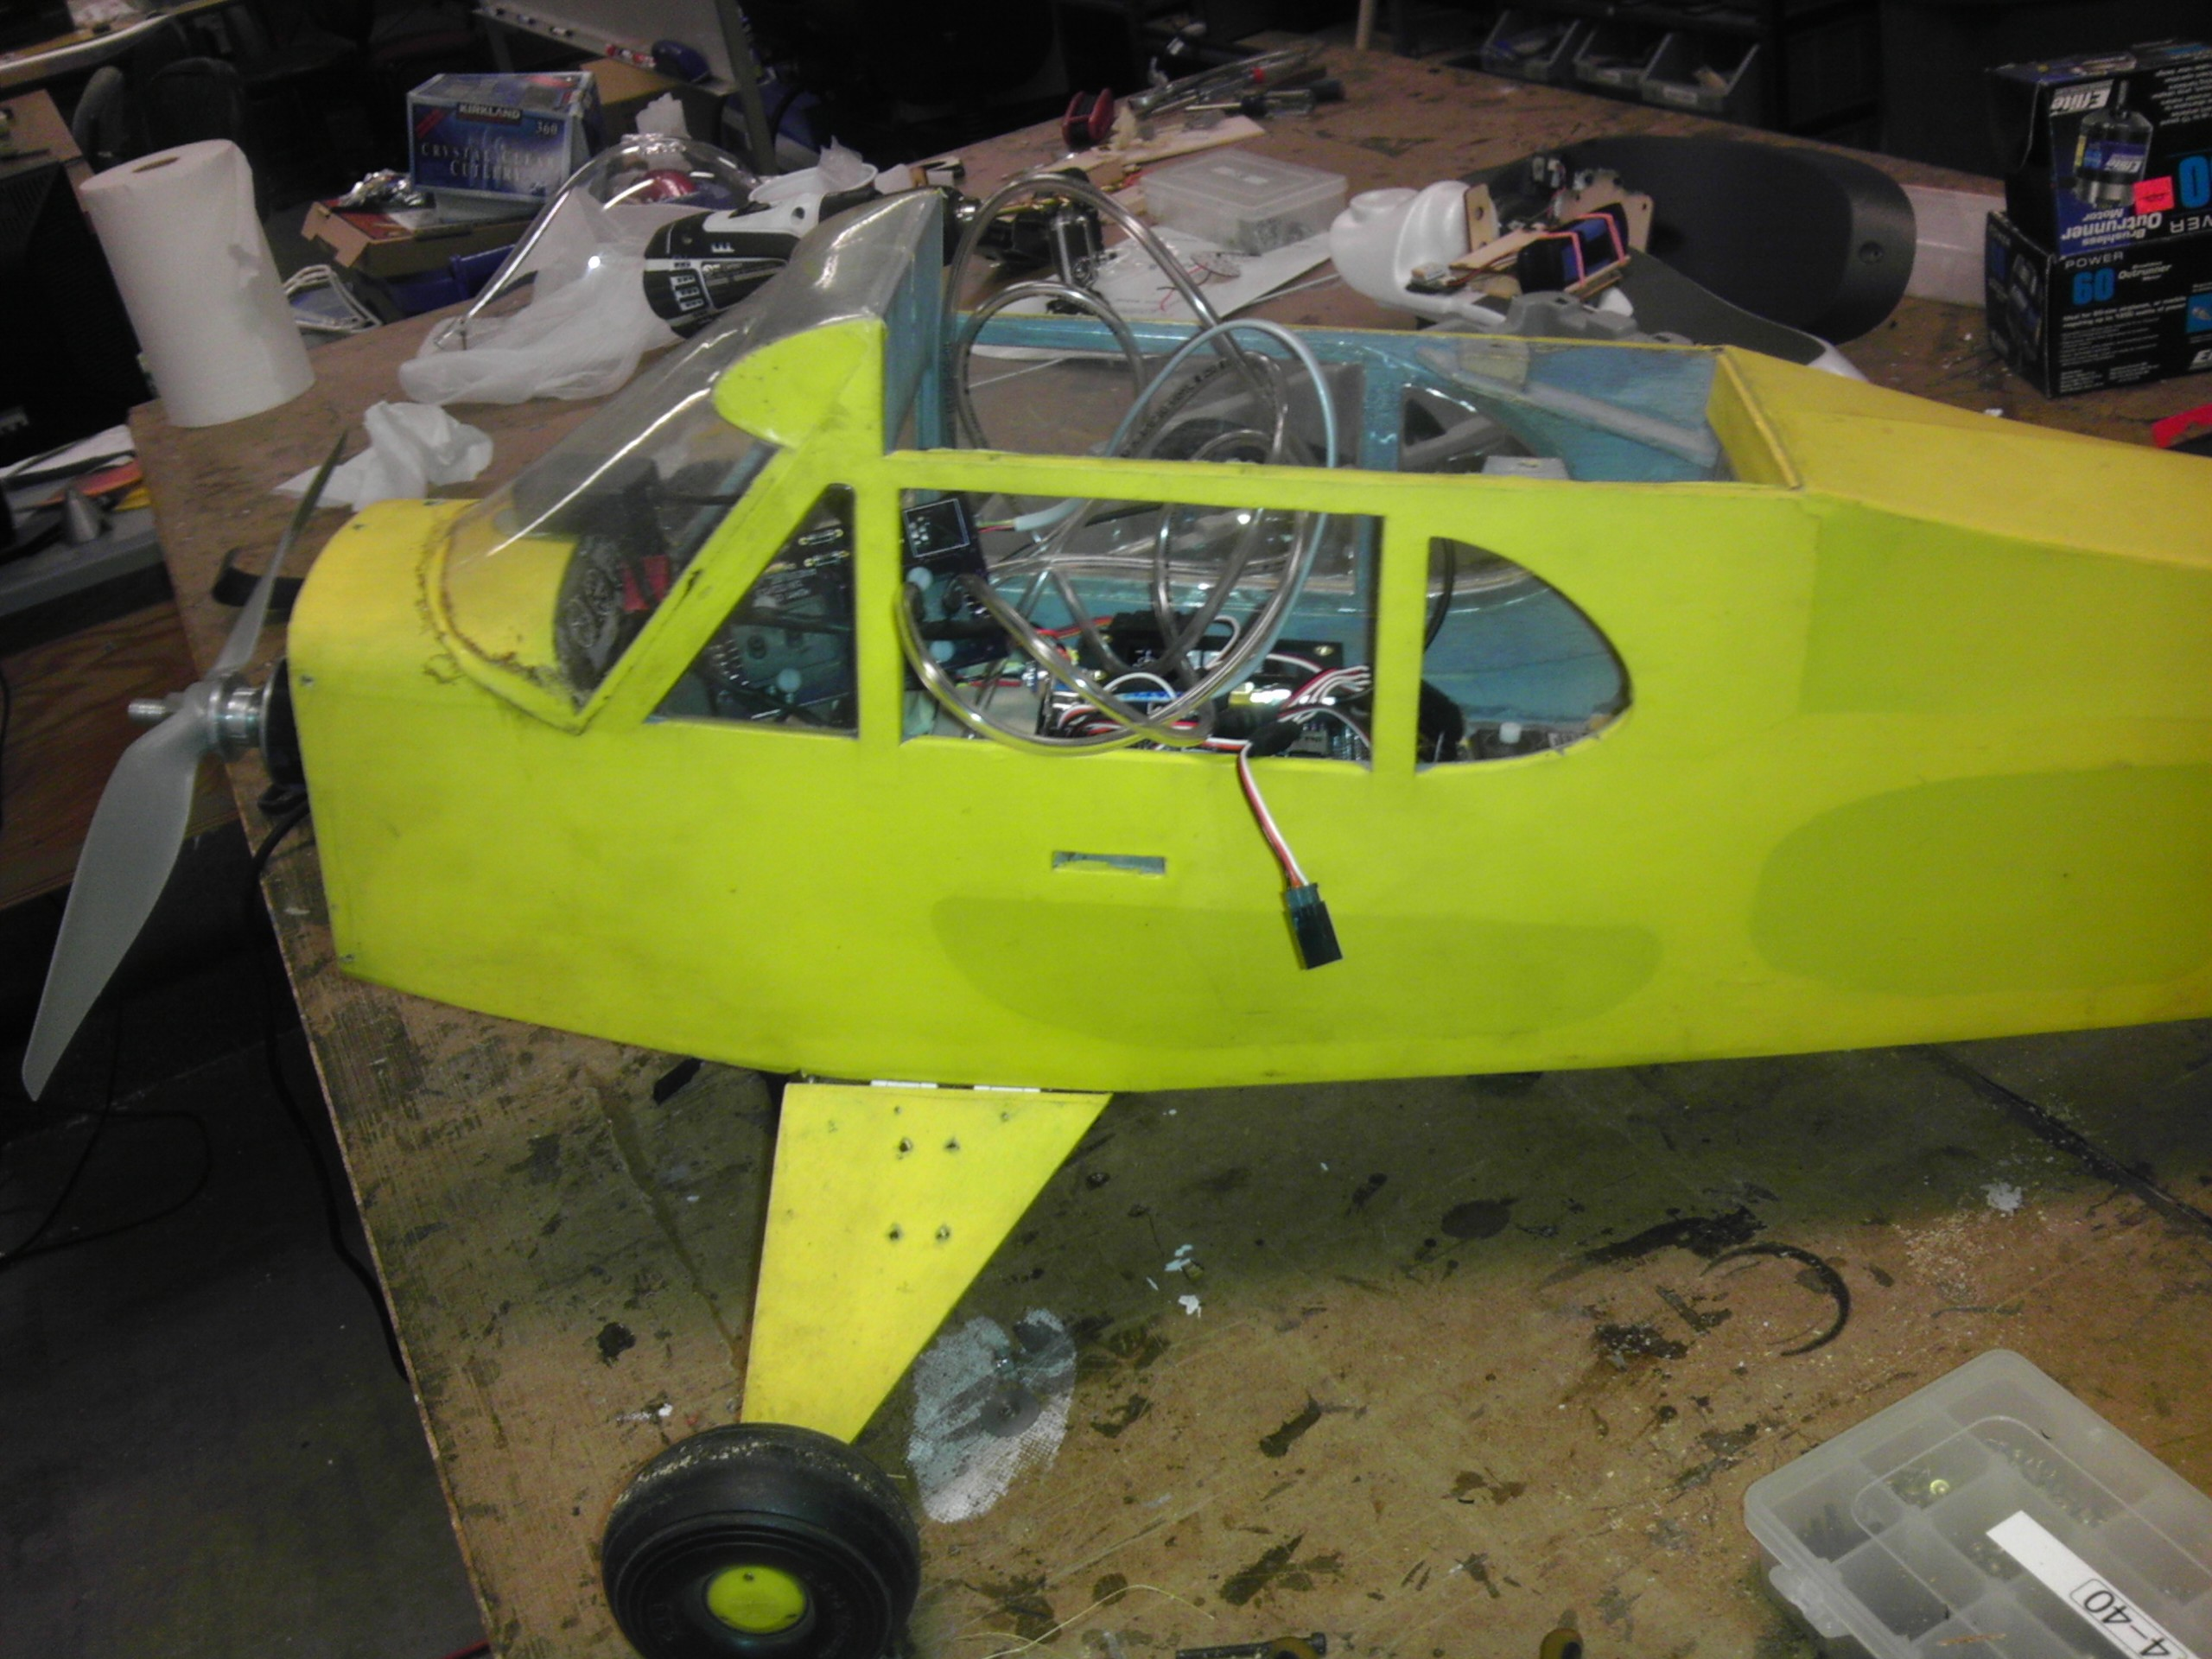
\includegraphics[width=0.9\textwidth]{figures/sysInt1.jpg}
\end{minipage}
\begin{minipage}[b]{0.45\linewidth}
  \centering
    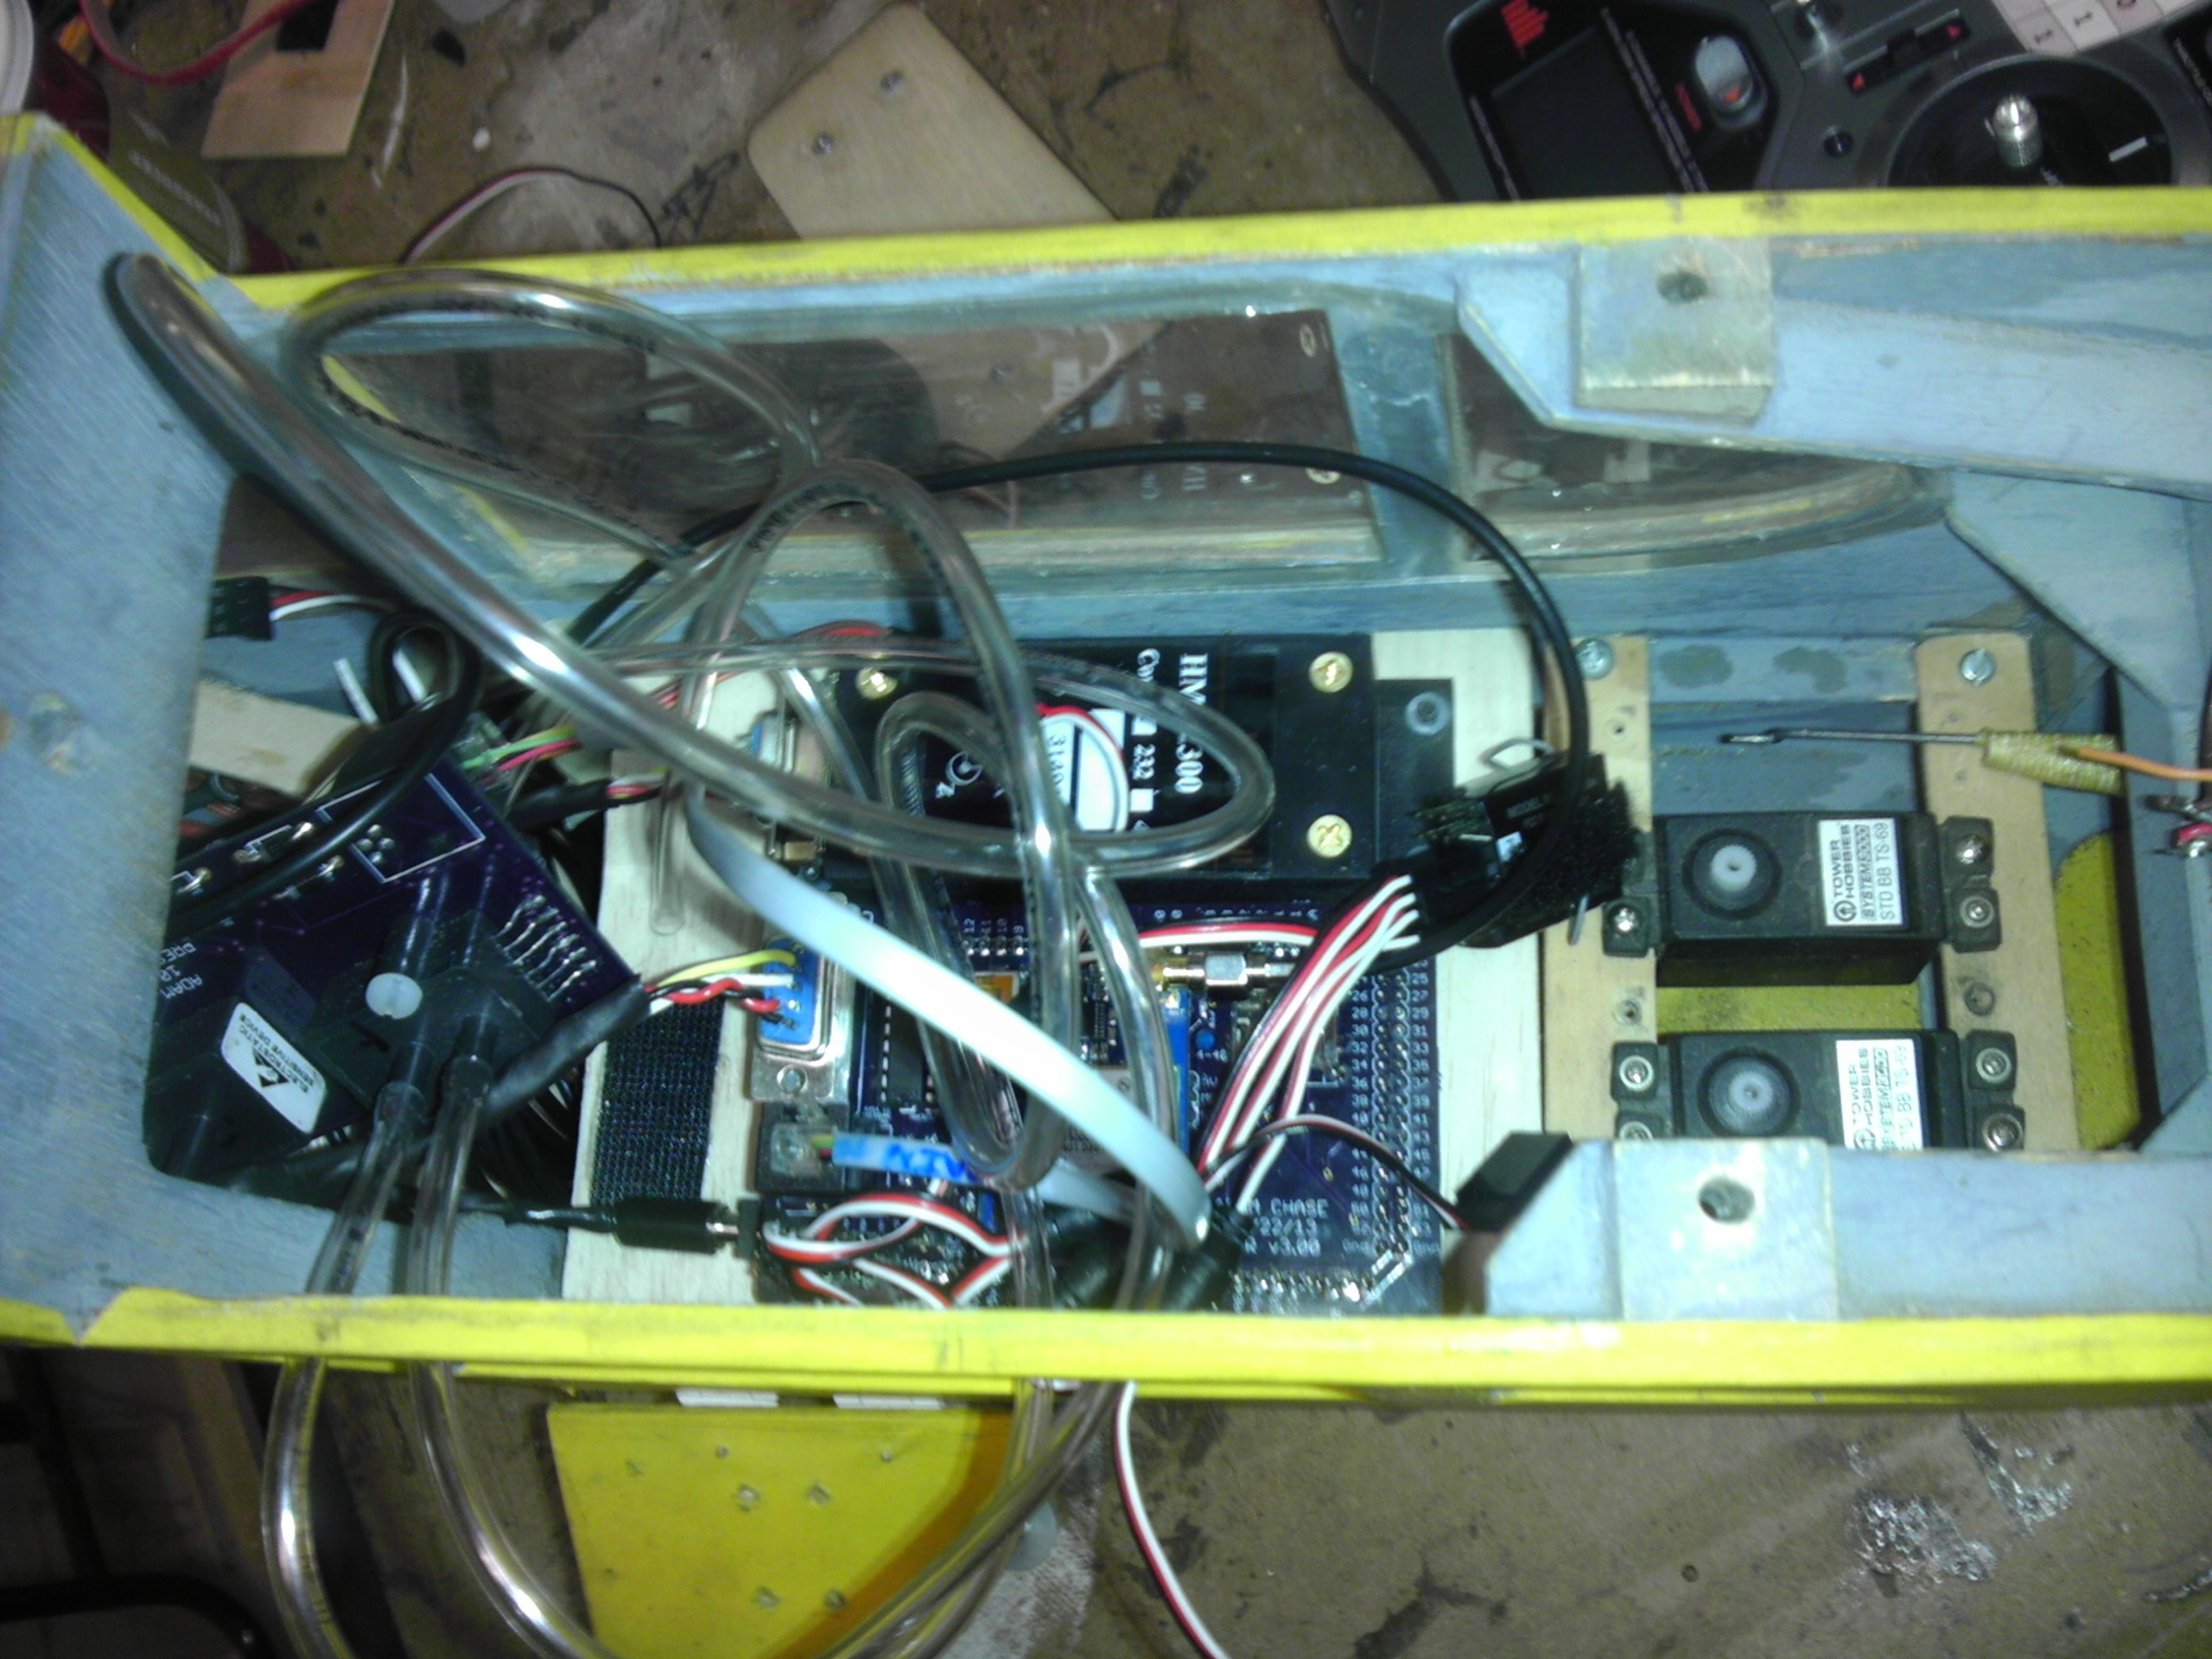
\includegraphics[width=0.9\textwidth]{figures/sysInt2.jpg}
\end{minipage}
\end{center}
\caption{System Integration into 0.40-size R/C Piper Cub}
\end{figure}
After integration, an initial test flight was conducted. Unfortunately, an electrical short-circuit caused the vehicle to  crash and corrupted some data, so no aerodynamic force estimation has been conducted. However, the micro-SD card did survive the crash, and provided enough data to show the system was collecting data as expected before the short-circuit.
\begin{figure}[H]
\label{sysIntPics}
\begin{center}
\begin{minipage}[b]{0.4\linewidth}
\label{preFlightFig}
  \centering
    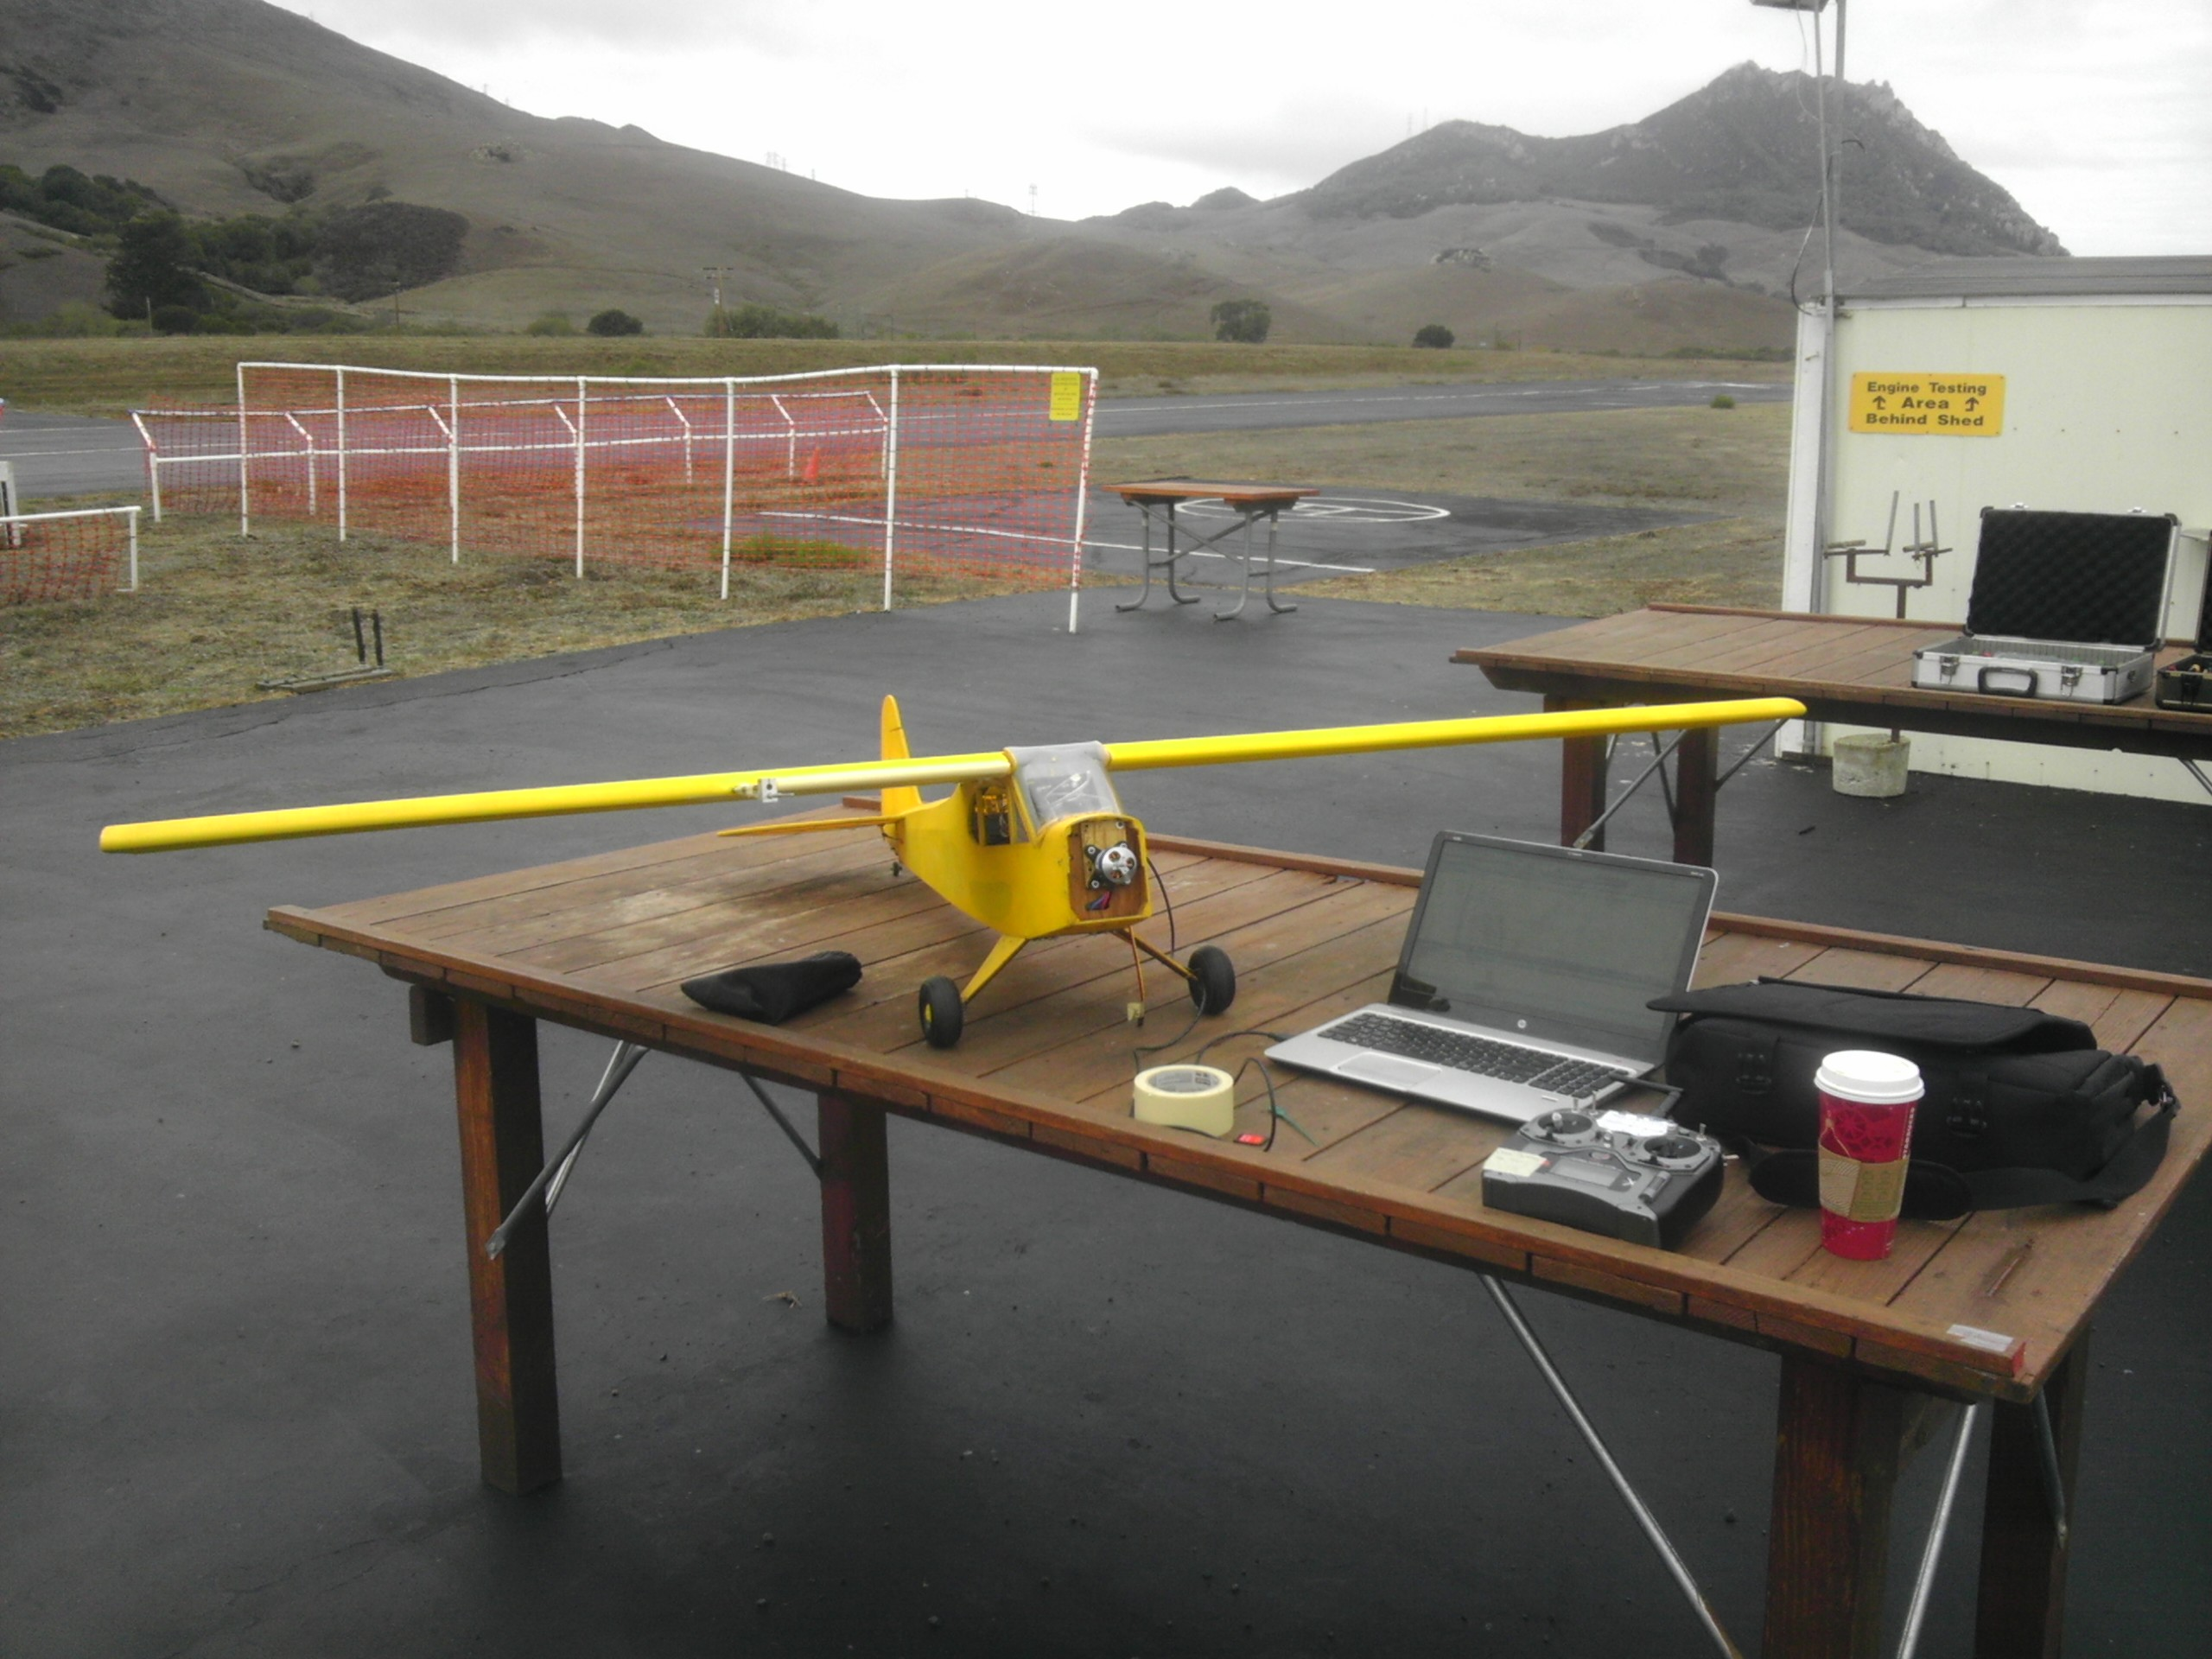
\includegraphics[width=0.9\textwidth]{figures/preFlight.jpg}
    \caption{Pre-Flight System Checks}
\end{minipage}
\begin{minipage}[b]{0.4\linewidth}
  \centering
    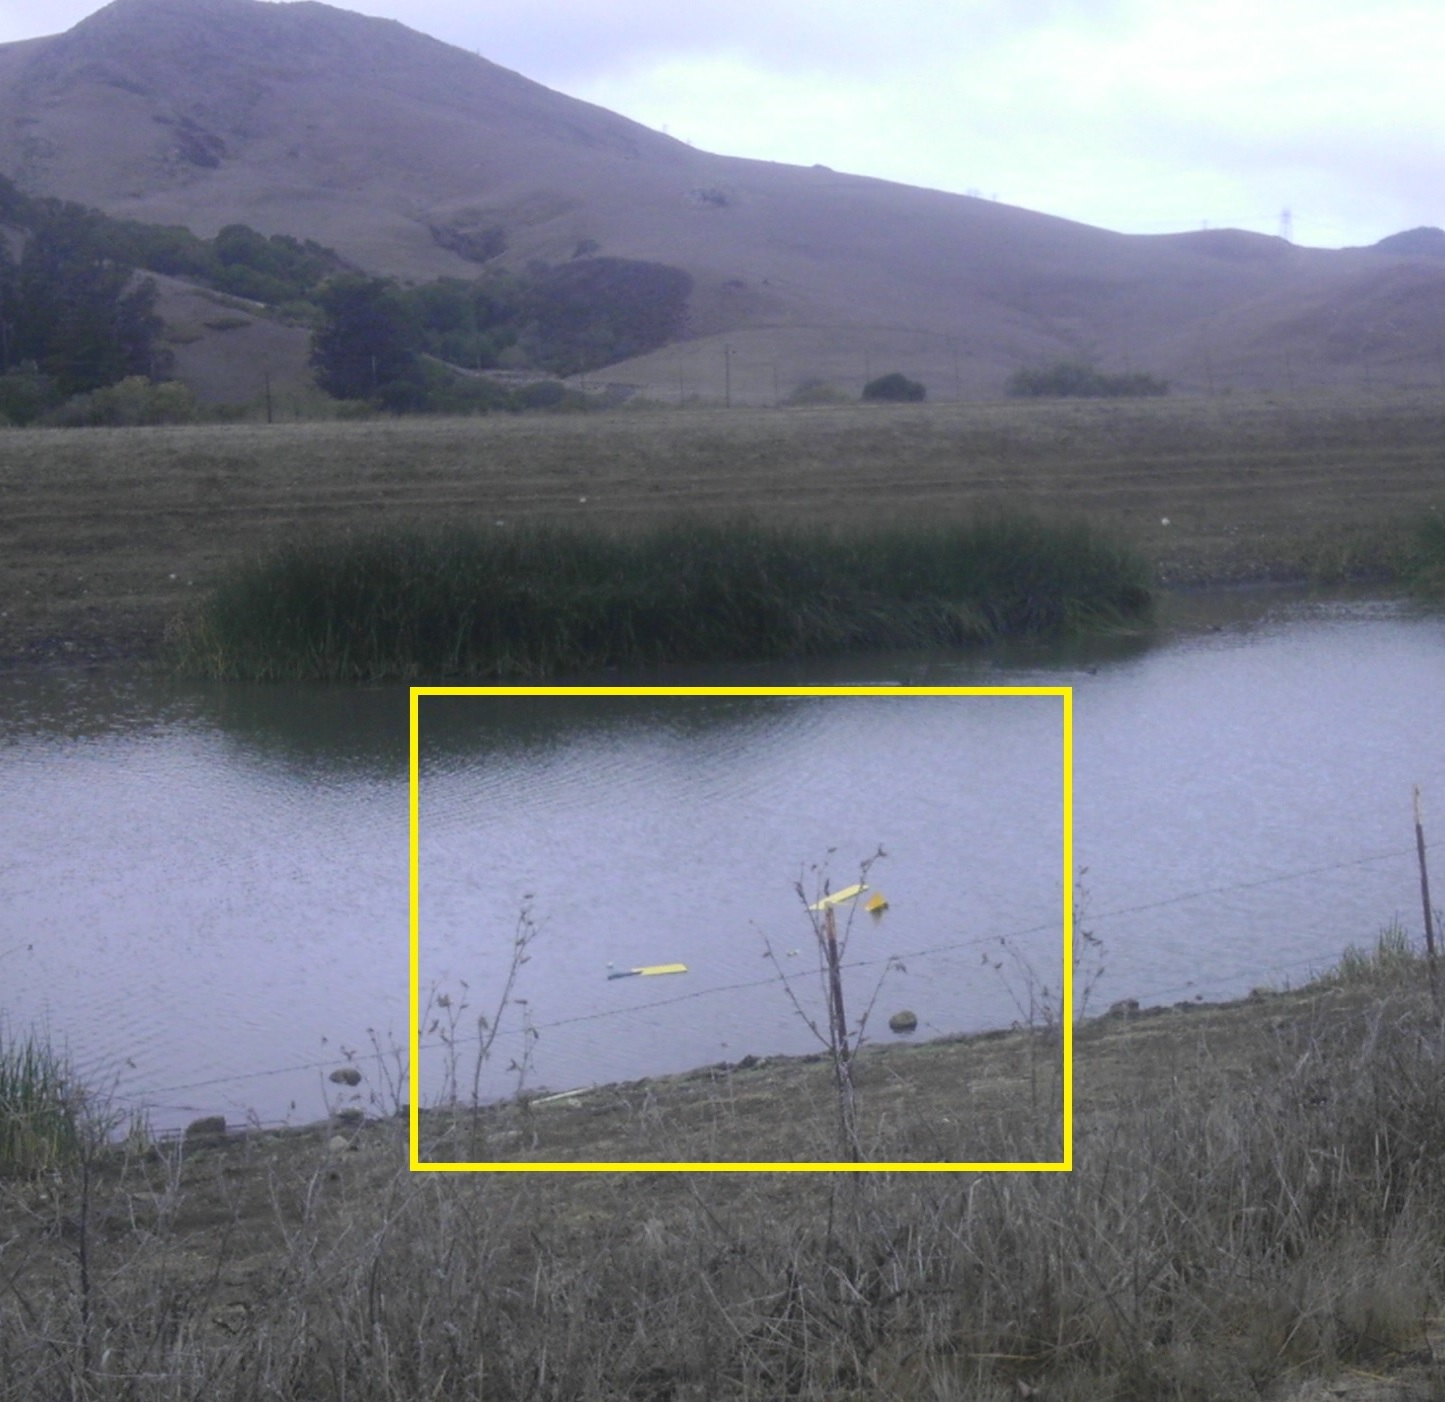
\includegraphics[width=0.9\textwidth]{figures/crash.jpg}
    \caption{Crashed Vehicle in Water}
\end{minipage}
\end{center}
\end{figure}

 The small amount of data collected was analyzed using a user interface developed to rapidly process the data acquisition system's files. This user interface will allow designers to analyze data immediately following a test flight and make corrections to the test flight program while still at the test flight location.
 
 Due to the vehicle crash, the accuracy of the system developed still needs to be extensively validated. The immediate future work following this paper will be quantifying the accuracy of the system, as well as verifying reliability and safe integration into multiple unmanned systems. Most of the accuracy estimation will be accomplished by measuring changes to a vehicle's drag polar. The ability to measure parasite drag will be proven by adding payloads with a known drag coefficient to ``dirty'' the aircraft, and then measuring the change in the parasite drag coefficient of the test vehicle. To quantify the accuracy of drag-due-to-lift measurement, wings with different aspect ratios will be used on the vehicle, which should combine into a single equivalent curve\cite{prandtl1923applications}. Following the accuracy estimation, a sensor fusion algorithm will be developed to combine inertial sensors with the air data system and other available sensors in a manner similar to other current research,\cite{wvINSAirData}$^,$\cite{gtUKF} in order to give full situational awareness to the UAS. This situational awareness could allow stability and control derivative estimation, which the aircraft designer could use to size tail and control surfaces.